\documentclass[11pt]{article}
\usepackage[margin=0.7in]{geometry}
\usepackage{multirow}
\usepackage {graphicx}
\usepackage[utf8x]{inputenc} % указать кодировку русского текста
\usepackage[russian]{babel} % указать, что язык текста - русский
\usepackage{fancyhdr}
\pagestyle{fancy}
\usepackage{graphicx}
\graphicspath{{pictures/}}
\DeclareGraphicsExtensions{.pdf,.png,.jpg}
\usepackage{tocloft}
\renewcommand{\cftsecleader}{\cftdotfill{\cftdotsep}}
\begin{document}
\begin{titlepage}
\begin{center}
\large\textbf{Московский Физико-Технический Институт}\\
\large\textbf{(государственный университет)}
\vfill
\huge\textbf{ Работа 3.2.4}\\
\huge\textbf{Свободные колебания в электрическом контуре}\\
\vfill
\large Факультет электроники, фотоники и молекулярной физики\\
\end{center}
\end{titlepage}
\fancyhead[L] {Работа 3.2.4}
\tableofcontents
\newpage
\section{Цель работы:}
Исследование свободных колебаний в электрическом колебательном контуре.\\
\textbf{В работе используются}:\\ генератор импульсов, электронное реле, магазин сопротивлений, магазин ёмкостей, индуктивность, электронный осциллограф, унивенрсальный мост, магазин сопротивлений.
\section{Теория}
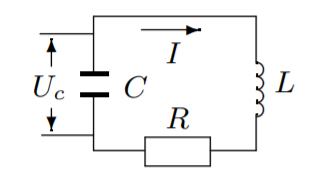
\includegraphics[width=10cm]{g1}\\
Рассмотрим электрический контур, состоящий из последовательно соединённых конденстора $C$, катушки индуктивности $L$ и резистора $R$. Обозначим разность потенциалов на конденсаторе $U_C$, а ток, текущий в контуре, через $I$. \\
Сумма падений напряжения на элементах цепи в отсутствие внешней ЭДС равна нулю:\\
$$RI + U_c + L\frac{dI}{dt} = 0$$\\
Подставим $I = C\frac{dU_c}{dt}$\\
$$CL\frac{d^2U_c}{dt^2} + CR\frac{dU_c}{dt} + U_c = 0$$\\
Разделим это уравнение на $CL$ и введем обозначения:\\
$\gamma = \frac{R}{2L}$, $\omega_{0}^2 = \frac{1}{LC}$\\
Тогда уравнение примет вид:\\
$$\frac{d^2U_c}{dt^2} + 2\gamma\frac{dU_c}{dt} + \omega_{0}^2U_{c} = 0$$\\
Для решения уравнения введем вспомогательную переменную $U(t)$, положив 
$$U_c(t) = U(t)\exp^{-\gamma t}$$
При этом получим уравнение:
$$\frac{d^2U}{dt^2} + \omega_{1}^2U = 0$$ где $\omega_{1}^2 = \omega_{0}^2 - \gamma^2$\\
В зависимости от соотношения между коэффициентом затухания $\gamma$ и собственной частотой $\omega_{0}$ решение $U(t)$ уравнения и соответственно напряжение на конденсаторе по-разному меняется от времени. Возможны три варианта, один из которых (затухающие колебания), нам и нужен. \\
\section{Описание установки}

На рисунке приведена схема для исследования свободных колебаний в контуре, содержащем постоянную индуктивность $L$ и переменные ёмкость $C$ и сопротивление $R$. Колебания наблюдаются на экране осциллографа.\\
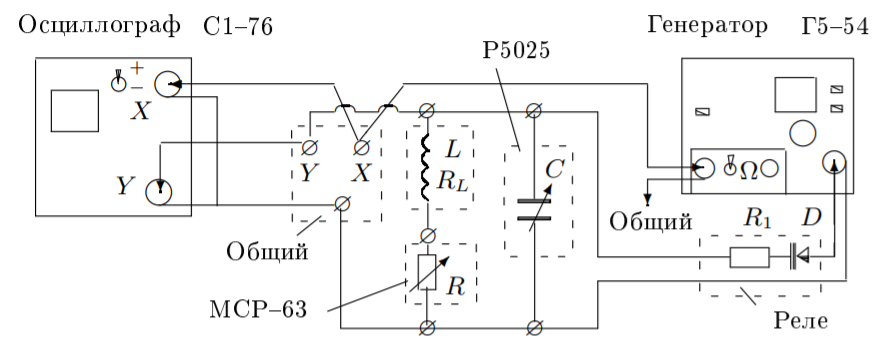
\includegraphics[width=14cm]{g2}\\
Для периодического возбуждения колебаний в контуре используется генератор импульсов Г5-54. С выхода генератора по коаксиальному кабелю импульсы поступают на колебательный контур через электронное реле, смонтированное в отдельном блоке (или на выходе генератора). Реле содержит тиристор $D$ и ограничительный резистор $R_1$.\\
Импульсы заряжают конденсатор $C$. После каждого импульса генератор отключается от колебательного контура, и в контуре возникают свободные затухающие колебания. Входное сопротивление осциллографа велико ($\approx 1$ МОм), так что его влиянием на контур можно пренебречь. Для получения устойчивой картины затухающих колебаний используется режим ждущей развёртки с синхронизацией внешними импульсами, поступающими с выхода <<синхроимпульсы>> генератора.
\section{Ход работы}
\subsection{Измерение периодов свободных колебаний}
Соберем полную схему, представленную на рисунке выше. Установим на магазине сопротивлений величину $R = 0$, на магазине ёмкостей - величину $C = 0,02$ мкФ. Изменяя ёмкость С от 0,02 мкФ до 0,9 мкФ, проведем измерения значений периодов Т свободных колебаний.\\
$T_0 = \frac{1}{f} = 0,01$ сек. Период рассчитаем по формуле $T = \frac{T_{0}x}{nx_{0}}$.\\ Тут же сопоставим каждому из значений $C$ значения периода, вычисленные теоретически по формуле $T = 2\pi\sqrt{LC}$.\\
Проверим также, что $L \approx 0,2$ Гн, как и говорилось в описании к работе.\\
Рассчитаем погрешность определения $T_{teor}$:\\
$$(\frac{\sigma_T}{T})^2 = (\frac{\sigma_x}{x})^2 + (\frac{\sigma_{x_0}}{x_0})^2$$\\
$$(\frac{\sigma_T}{T})^2 = (\frac{0,2}{4,358})^2 + (\frac{0,2}{9,48})^2 \approx 0,002 + 0,000445 \approx 0,002445$$\\
$$\sigma_{T_{exp}} = 0,086 \; ms$$\\
\begin{center}
\begin{tabular}{|c|c|c|c|c|c|}\\
\hline
$C$, мкФ & $x_0$ & $x$ & $n$ & $T_{exp}$, мс & $T_{teor}$, мс\\
\hline
0,02 & 9,4 & 1,58 & 4 & 0,42 & 0,397\\
\hline
0,024 & 9,5 & 1,73 & 4 & 0,456 & 0,435\\
\hline
0,028 & 9,5 & 1,88 & 4 & 0,495 & 0,47\\
\hline
0,09 & 9,5 & 1,68 & 2 & 0,88 & 0,84\\
\hline
0,1 & 9,5 & 3,55 & 4 & 0,934 & 0,888\\
\hline
0,15 & 9,5 & 4,35 & 4 & 1,445 & 1,088\\
\hline
0,2 & 9,5 & 3,75 & 3 & 1,316 & 1,256\\
\hline
0,25 & 9,5 & 4,2 & 3 & 1,474 & 1,404\\
\hline
0,3 & 9,5 & 4,6 & 3 & 1,614 & 1,538\\
\hline
0,35 & 9,5 & 4,9 & 3& 1,719 & 1,662\\
\hline
0,4 & 9,5 & 3,5 & 2 & 1,842 & 1,776\\
\hline
0,45 & 9,4 & 3,7 & 2 & 1,968 & 1,884\\
\hline
0,5 & 9,4 & 3,95 & 2 & 2,101 & 1,986\\
\hline
0,55 & 9,4 & 4,1 & 2 & 2,18 & 2,083\\
\hline
0,6 & 9,5 & 4,35 & 2 & 2,289 & 2,175\\
\hline
0,65 & 9,5 & 4,5 & 2 & 2,368 & 2,264\\
\hline
0,7 & 9,5 & 4,7 & 2 & 2,473 & 2,35\\
\hline
0,75 & 9,5 & 7,2 & 3 & 2,526 & 2,432\\
\hline
0,8 & 9,5 & 7,5 & 3 & 2,632 & 2,512\\
\hline
0,85 & 9,5 & 7,8 & 3 & 2,737 & 2,589\\
\hline
0,9 & 9,5 & 8 & 3 & 2,807 & 2,664\\
\hline
\end{tabular}\\
\end{center}
Построим график $T_{exp} = f(T_{teor})$.\\
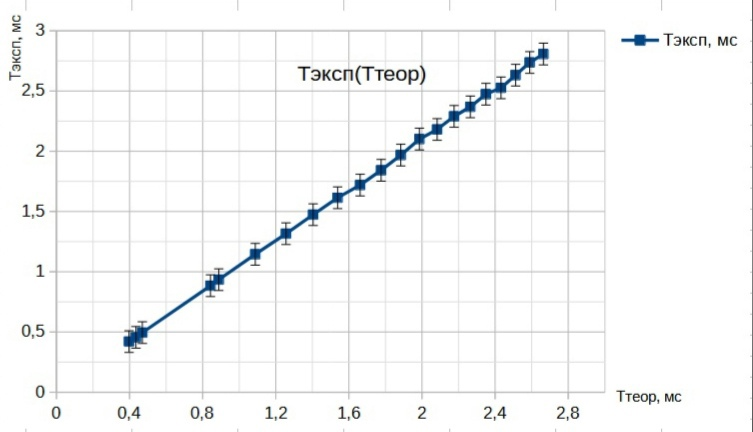
\includegraphics[width=18cm]{g4}\\
\subsection{Критическое сопротивление и декремент затухания}
1) Считая $L \approx 200$ мГн, рассчитаем $C$, при которой $\nu_0 = 1/2\pi \sqrt{LC} = 5$ кГц. Критическое сопротивление в этом случае $R_{кр} = 2\sqrt{\frac{L}{C}} \approx 12,6$ кОм. Рассчитаем логарифмический декремент затухания $\theta = \frac{1}{n}ln\frac{U_k}{U_{k+n}}$ в диапазоне $(0.1 - 0.3)R_{кр}$:\\
\begin{table}[h]
\centering
\begin{tabular}{|c|c|c|c|c|c|c|c|c|}
\hline
$R$, Ом     & 1000 & 1400 & 1800 & 2200 & 2600 & 2800 & 3000\\
\hline
$2U_k$ & 2,8 & 1,95 & 1,52 & 1,16 & 0,92 & 0,8 & 0,7\\ \hline
$2U_{k+n}$ & 0,6 & 0,4 & 0,22 & 0,12 & 0,23 & 0,18 & 0,14\\ \hline
$n$ & 2 & 2 & 2 & 2 & 1 & 1 & 1 \\ \hline
$\theta$ & 0,77 & 0,79 & 0,966 & 1,134 & 1,386 & 1,492 & 1,61\\ \hline
$\sigma_{\theta}$ & 0,06 & 0,1 & 0,22 & 0,47 & 0,31 & 0,42 & 0,58\\
\hline
\end{tabular}
\caption{Зависимость $\theta = \theta(R)$.}
\end{table}\\
Погрешность вычисления $\theta$ находили по формуле:\\
$$\sigma_{\theta} = \theta \sqrt{\frac{\sigma_{U_k}}{U_k}^2 + \frac{\sigma_{U_{k+n}}}{U_{k+n}}^2}$$\\
2) Получив изображение колебаний на фазовой плоскости (в координатах $\left(U_C, \frac{dU_C}{dt}\right)$, убеждаемся, что декремент затухания вычисленный по тем же способом с достаточной точностью совпадает с вычисленным в кооридинатах $\left( U_C, t\right)$.\\
\begin{table}[h]
\centering
\begin{tabular}{|c|c|c|c|c|c|c|c|c|}
\hline
$R$, Ом     & 1000 & 1400 & 1800 & 2200 & 2600 & 2800 & 3000\\
\hline
$2x_k$ & 1,6 & 2,3 & 2,75 & 3,15 & 3,5 & 3,6 & 1,9\\ \hline
$2x_{k+n}$ & 0,6 & 0,5 & 0,4 & 0,3 & 0,2 & 0,15 & 0,4\\ \hline
$n$ & 2 & 2 & 2 & 2 & 2 & 2 & 1 \\ \hline
$\theta$ & 0,49 & 0,763 & 0,964 & 1,176 & 1,431 & 1,589 & 1,558\\ \hline
$\sigma_{\theta}$ & 0,006 & 0,01 & 0,02 & 0,07 & 0,08 & 0,14 & 0,07\\
\hline
\end{tabular}
\caption{Зависимость $\theta = \theta(R)$.}
\end{table}\\

3) Измеряем индуктивность $L$ и $R_L$ катушки для трёх значений частоты:\\
\begin{table}[h]
\centering
\begin{tabular}{|c|c|c|c|}
\hline
$f$, Гц  & 50    & 1000  & 5000  \\ \hline
$R_L$, Ом & 11.122 & 18.720 & 38.5 \\ \hline
$L$, мГн & 204.51 & 199.95 & 200 \\ \hline
\end{tabular}
\caption{Значения $R_L$ и $L$ катушки при разных частотах.}
\end{table}\\
4) Будем считать, что сопротивление катушки пропорционально частоте:\\
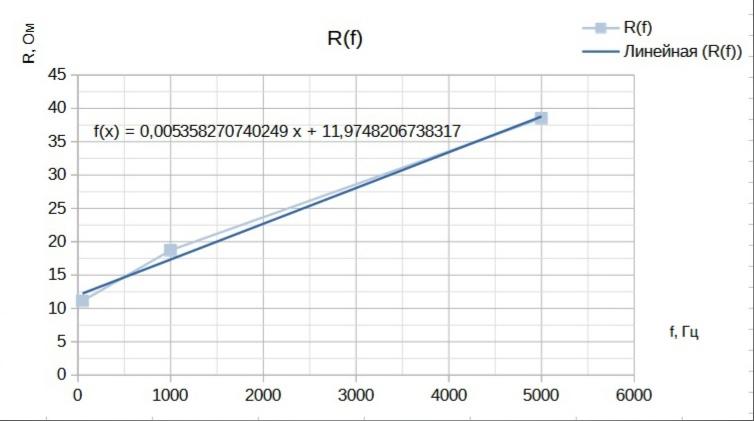
\includegraphics[width=15cm]{g5}\\
\\
Тогда можно вычислить суммарное сопротивление контура: $R_{sum} = R + R_L$\\
5) Построим график в координатах $\frac{1}{\theta^2} = f(\frac{1}{R_{sum}^2})$.\\
Занесём все необходимые данные в таблицу:
\begin{table}[h]
\centering
\begin{tabular}{|c|c|c|c|c|c|c|c|}
\hline
$\frac{1}{\theta^2}$ & 1,686 & 1,594 & 1,07 & 0,778 & 0,520 & 0,450 & 0,386\\ \hline
$\sigma_{\frac{1}{\theta^2}}$ & 0,287 & 0,407 & 0,492 & 0,651 & 0,233 & 0,256 & 0,281\\ \hline 
$\frac{1}{R_{sum}^2}$ & 9,75 & 5,01 & 3,04 & 2,04 & 1,47 & 1,26 & 1,10\\ \hline
\end{tabular}
\caption{Зависимость $\frac{1}{\theta^2} = f(\frac{1}{R_{sum}^2})$ }
\end{table}\\
Погрешность $\sigma_{\frac{1}{\theta^2}}$ считали по формуле:\\
$$ \sigma_{\frac{1}{\theta^2}} = \frac{2}{\theta^2}\frac{\sigma_{\theta}}{\theta}$$\\
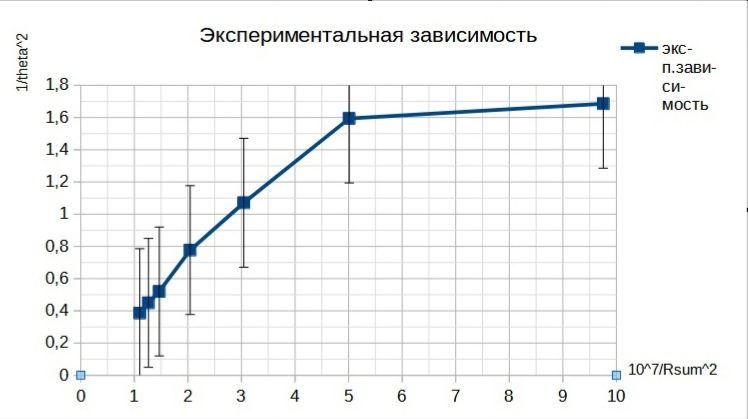
\includegraphics[width=15cm]{g6}\\
По наклону графика вблизи начала координат определим $R_{kr} = 2\pi\sqrt{\triangle Y / \triangle X}$\\
$R_{kr} \approx 2\cdot 3,14 \cdot 0,616 \cdot 3162,3 \approx 12,2$ кОм.\\
Погрешность вычисляем по формуле:\\
$$\sigma_{R_{kr}} = \frac{1}{2}R_{kr}\frac{\sigma_{a}}{a} \approx 0,3$$ кОм.\\
Тогда итоговый ответ для $R_{kr}$, найденного из графика: \fbox{$R_{kre} = 12,2 \pm 0,3 \; kOm$ }\\
6) Сравним этот ответ с теоретическими выкладками:\\
$R_{kr} = 2\sqrt{L/C}$, $C = 5$ нФ, $L \approx 0,2$ Гн.\\
$$R_{kr} = 2\sqrt{0,2*10^9/5} \approx 12,6 \; kOm$$\\
Погрешность вычисляем по формуле:\\
$$\sigma_{R_{kr}} = \frac{1}{2}R_{kr}\frac{\sigma_{L}}{L} \approx 0,3$$.\\
Тогда итоговый ответ для $R_{kr}$, вычисленного теоретически: \fbox{$R_{krt} = 12,6 \pm 0,3 \; kOm$ }\\
Видим, что полученные результаты для экспериментального и теоретического значения различаются всего на $2,4\%$.\\
\subsection{Добротность}
1) Рассчитаем добротность контура $Q$ для максимального и минимального значений $\theta$ по картине затухающих колебаний и сравним с расчётом $Q$ через параметры контура $Q = \frac{1}{R}\sqrt{\frac{L}{C}}$\\
Берем максимум и минимум сопротивления из второй таблицы. Погрешность определения добротности рассчитываем по формуле:\\
$$\sigma_{Q} = \frac{1}{2}Q\frac{\sigma_{L}}{L}$$
$$ R_{min} = 1000 \; Om \; \; \; Q = 6,31 \pm 0,02$$
$$ R_{max} = 3000 \; Om \; \; \; Q = 2,11 \pm 0,01$$
2) Рассчитаем добротность $Q = \frac{\pi}{\theta}$ по спирали на фазовой плоскости: \\
Аналогично возьмем минимум и максимум декремента из третьей таблицы. Погрешность вычисления добротности составит:\\
$$\sigma_{Q} = Q\frac{\sigma_{\theta}}{\theta}$$
$$ \theta_{min} = 0,49;  \; \; \; Q = 6,41 \pm 0,08$$
$$ \theta_{max} = 1,589; \; \; \; Q = 1,98 \pm 0,17$$
По затуханию на обычной плоскости:\\
$$\sigma_{Q} = Q\frac{\sigma_{\theta}}{\theta}$$
$$ \theta_{min} = 0,77;  \; \; \; Q = 4,01 \pm 0,31$$
$$ \theta_{max} = 1,61; \; \; \; Q = 1,95 \pm 0,71$$
Сведем результаты двух экспериментов в таблицы:\\
\begin{table}[h]
\centering
\begin{tabular}{|c|c|c|c|}
\hline
$L$ & $R_{kr}$ теор. & $R_{kr}$ эксп & \\ \hline
$200$ мГн &$12,6 \pm 0,3$ Ом & $12,2 \pm 0,3$ Ом & \\ \hline
$R$ & $Q$ теор. & $f(\theta)$ & Спираль\\ \hline
$1000$ Ом & $6,31 \pm 0,02$ &$4,01 \pm 0,31$ & $6,41 \pm 0,08$ \\ \hline
$3000$ Ом & $2,11 \pm 0,01$ & $1,95 \pm 0,71$ & $1,98 \pm 0,17$ \\ \hline
\end{tabular}
\caption{Критическое сопротивление и добротность контуров с наибольшим и наименьшим затуханием}
\end{table}
\section{Вывод}
В данной работе мы исследовали свободные колебания в электрическом колебательном контуре, а также вычислили некоторые из его параметров: добротность, логарифмический декремент, а также критическое сопротивление для разных параметров контура.\\
Основные результаты эксперимента приведены в таблице 5. Из неё видно, что результаты теоретического и экспериментальных значений критического сопротивления сходятся довольно точно, а вот значение добротности, как $f(\theta)$ оказалось далеко от двух других, одно из которых теоретическое, а другое - экспериментальное. \\
\end{document}